\documentclass[12pt]{article}

\usepackage{amsmath}
\usepackage{amssymb}
\usepackage{amsthm}

\usepackage{geometry}

\usepackage{tikz}
\usetikzlibrary{arrows,automata}

\title{CS321 - Notes}
\author{Trevor Bramwell}
\date{Fri Oct 11 12:17:02 PDT 2013}

\begin{document}
\maketitle

\section*{NFAs (Cont.)}

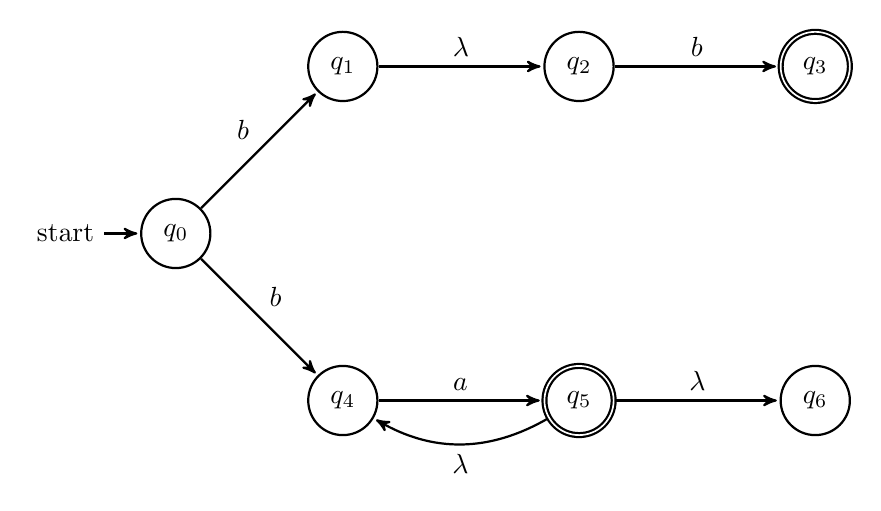
\begin{tikzpicture}[->,>=stealth',shorten >=1pt,auto,node distance=3cm,
                    thick]
  \tikzstyle{every state}=[fill=white]

  \node[state,initial]   (A)              {$q_0$};
  \node[state]           (B) [above right of=A] {$q_1$};
  \node[state]                     (C) [right of=B] {$q_2$};
  \node[state,accepting]                     (D) [right of=C] {$q_3$};
  \node[state]                     (E) [below right of=A] {$q_4$};
  \node[state,accepting]                     (F) [right of=E] {$q_5$};
  \node[state]                     (G) [right of=F] {$q_6$};

  \path (A) edge node {$b$} (B)
            edge node {$b$} (E)
        (B) edge node {$\lambda$} (C)
        (C) edge node {$b$} (D)        
        (E) edge node {$a$} (F)
        (F) edge [bend left] node {$\lambda$} (E)
            edge node {$\lambda$} (G);
\end{tikzpicture}

\subsection*{Transition Functions}

\begin{align*}
    \delta^*(q_0, \lambda) &= \{q_0\}\\
    \delta^*(q_1, \lambda) &= \{q_1, q_2\}\\
    \delta^*(q_0, ba) &= \{q_4, q_5, q_6\}\\
    \delta^*(q_1, bbb) &= \emptyset
\end{align*}

Define $L(N)$, $N$ is an NFA.

$L(N) = \{ w : w \in \Sigma^*,\delta^*(q_0, w) \cap F \ne \emptyset\}$

There is at least one final state in the set can be written:
$\delta^*(q_0,w) \cap F \ne \emptyset$
or
$|\delta^*(q_0,w) \cap F| \ge 1$.

%

$L = \{ab, aba\}^*$
\begin{align*}
    \lambda &\in L
  ab aba ab &\in L
\end{align*}

%
%
% -> O -a> O -b> O
%

\end{document}
